\section*{Problem 1}
The plots for problem 1 below, the code is in the appendix.
\begin{figure}[h]
    \centering
    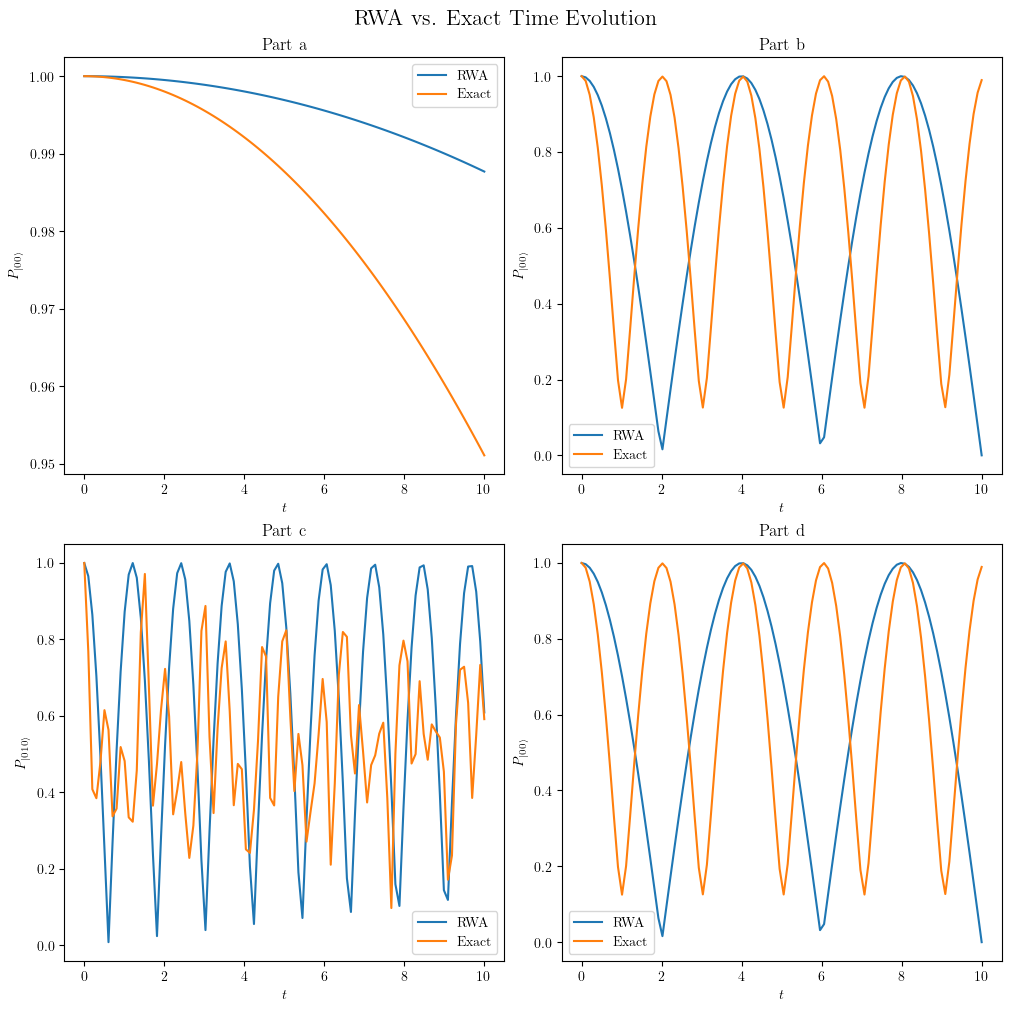
\includegraphics[width=1\linewidth]{Resources//245//Homework 7/245 Homework 7 Problem 1.png}
    \label{fig:enter-label}
\end{figure}
I plotted the RWA and exact time evolution on the same graphs.

\pagebreak
\section*{Problem 2}
The graphs for parts $i$ through $vi$ are below. Of particular interest are $v$ and $vi$. For part $v$ we do expect some fluctuations outside of the $8$th level, it's difficult to see because it is an order of magnitude smaller, but there is some probability of measuring the state $\ket{000}$.
\newpage

\vfill
\begin{center}
    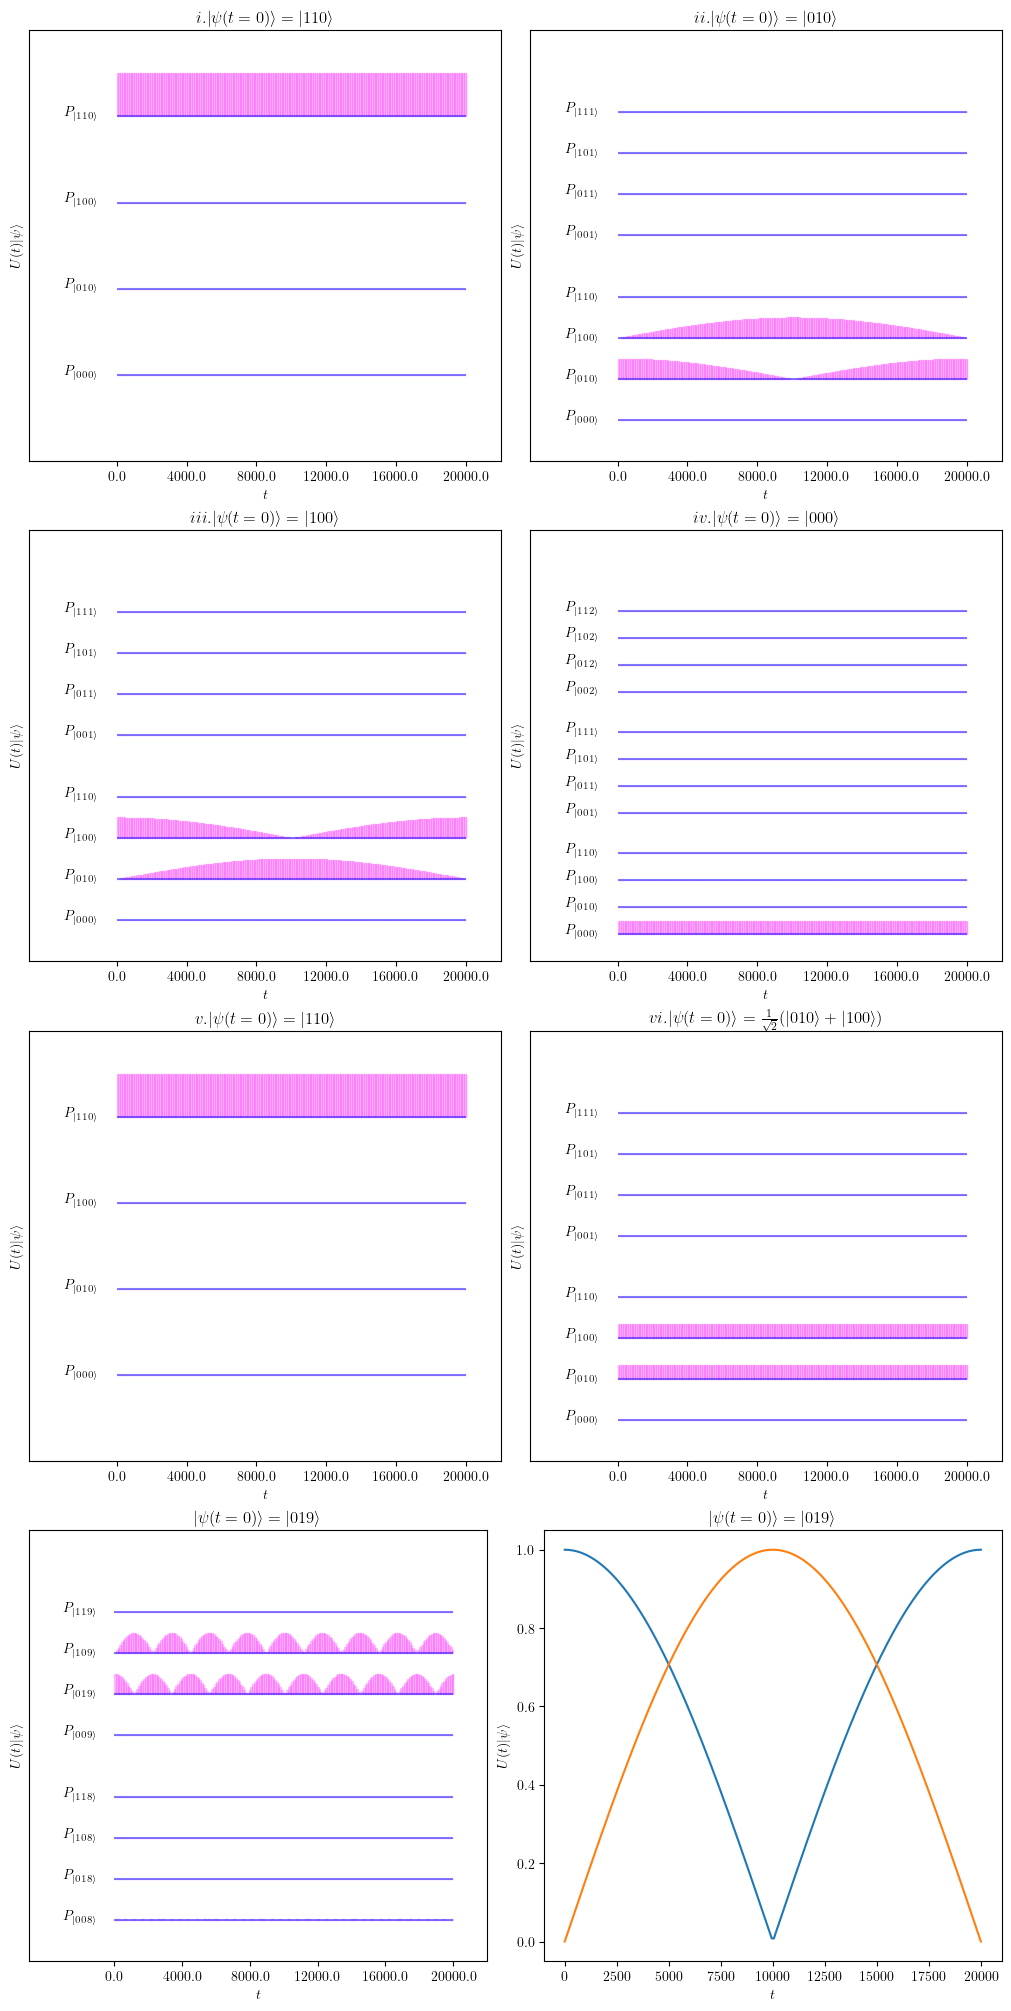
\includegraphics[width=1\linewidth]{Resources//245//Homework 7/245 Homework 7 Problem 2.png}
\end{center}
\vfill

\newpage
\pagebreak
\section*{Problem 3}
\subsection*{Part a}
Since the Hamiltonian commutes with itself, we can write down the time evolution operator as
\eq{
\hat{U}(t) &= e^{i g/2 t (\sigma_x\otimes \sigma_x)}\\
&= \sum_{k=0}^\infty \frac{(i g/2 t)^k}{k!} (\sigma_x\otimes \sigma_x)^k\\
&= \sum_{k=0}^\infty \frac{(i g/2 t)^k}{k!} \sigma_x^k\otimes \sigma_x^k\\
&= \sigma_x \otimes \sigma_x \sum_{k=0}^\infty \frac{(i g/2 t)^{2k+1}}{(2k+1)!}+\sigma_0 \otimes \sigma_0 \sum_{k=0}^\infty \frac{(i g/2 t)^{2k}}{(2k)!}\\
&= \sigma_x \otimes \sigma_x i \sum_{k=0}^\infty \frac{(-1)^{k}}{(2k+1)!}( g/2 t)^{2k+1}+\sigma_0 \otimes \sigma_0 \sum_{k=0}^\infty \frac{(-1)^{k}}{(2k)!}( g/2 t)^{2k}\\
&= \sigma_x \otimes \sigma_x i \sin ( g/2 t) + \sigma_0 \otimes \sigma_0 \cos( g/2 t)
}

\subsection*{Part b}
The $XX_{(\chi)}$ gate is defined as
\eq{
XX(\chi) &\equiv -\sigma_x\otimes\sigma_x i \sin(\chi) + \sigma_0 \otimes \sigma_0 \cos(\chi)\\
&= \hat{U}( - 2/g \chi)
}
Equation (2) and (3) from the literature are
\eq{
RY(\theta) &\equiv \sigma_0 \cos(\frac{\theta}{2})-i\sigma_y\sin(\frac{\theta}{2})\\
RX(\theta) &\equiv \sigma_0 \cos(\frac{\theta}{2})-i\sigma_x\sin(\frac{\theta}{2})\\
}
Then we can write the CNOT gate as (3.1 Fig. 1) and we use QuTip to perform the matrix computation.
\eq{
CN &= RY^{(1)}(-\frac{\pi}{2})RX^{(1)}(-\frac{\pi}{2})RX^{(2)}(-\frac{\pi}{2})\hat{U}(-\frac{2}{g}\frac{\pi}{4})RY^{(1)}(\frac{\pi}{2})\\
&= \gamma \begin{bmatrix}
   1 & 0 & 0 & 0\\
   0 & 1 & 0 & 0\\
   0 & 0 & 0 & 1\\
   0 & 0 & 1 & 0
\end{bmatrix}
}
\pagebreak
\section*{Code Appendix}
\subsection*{Problem 1}
\begin{python}
def Hexact(g,w,w0,N):
    Hqubit = tensor((w0/2)*sz(),I(N))
    Hqho = w*(tensor(I(2),create(N)*destroy(N)) + 0.5)
    Hint = (g/2)*(tensor(sx(),create(N))+tensor(sx(),destroy(N)))
    return  Hqubit + Hqho + Hint

def Uexact(g,w,w0,N,t):
    return (-1j*Hexact(g,w,w0,N)*t).expm()

def Urwa(t,n,g,w,w0):
    Omega = (g/2)*sqrt(n+1)
    delta = w - w0
    Rabi = sqrt(Omega**2 + delta**2)
    
    return cos((Rabi/2)*t)*I(2) - 1j*(Omega/Rabi)*sin((Rabi/2)*t)*sx() - 1j*(delta/Rabi)*sin((Rabi/2)*t)*sz()

w = 2*pi
w0 = w
N = 20

tpoints = linspace(0,10,100)

plt.close('all')
fig1 = plt.figure(figsize=(10, 10), layout="constrained")
gs1_main = fig1.add_gridspec(2,2)

g = w/100
n = 0
psi1e = [absolute((Uexact(g,w,w0,N,t)*tensor(ket("0"),base(N,n))).full()[0]) for t in tpoints]
psi1 = [absolute((Urwa(t,n,g,w,w0)*ket("0"))[0]) for t in tpoints]
ax1 = fig1.add_subplot(gs1_main[0])
ax1.plot(tpoints,psi1)
ax1.plot(tpoints,psi1e)
ax1.legend(['RWA','Exact'])
ax1.set_xlabel("$t$")
ax1.set_ylabel("$P_{| 00 \\rangle}$")
ax4.set_title('$U(t) | 00 \\rangle$')


g = w/2
n = 0
psi2e = [absolute((Uexact(g,w,w0,N,t)*tensor(ket("0"),base(N,n))).full()[0]) for t in tpoints]
psi2 = [absolute((Urwa(t,n,g,w,w0)*ket("0"))[0]) for t in tpoints]
ax2 = fig1.add_subplot(gs1_main[1])
ax2.plot(tpoints,psi2)
ax2.plot(tpoints,psi2e)
ax2.legend(['RWA','Exact'])
ax2.set_xlabel("$t$")
ax2.set_ylabel("$P_{| 00 \\rangle}$")
ax4.set_title('$U(t) | 00 \\rangle$')


g = w/2
n = 10
psi3e = [absolute((Uexact(g,w,w0,N,t)*tensor(ket("0"),base(N,n))).full()[10]) for t in tpoints]
psi3 = [absolute((Urwa(t,n,g,w,w0)*ket("0"))[0]) for t in tpoints]
ax3 = fig1.add_subplot(gs1_main[2])
ax3.plot(tpoints,psi3)
ax3.plot(tpoints,psi3e)
ax3.legend(['RWA','Exact'])
ax3.set_xlabel("$t$")
ax3.set_ylabel("$P_{| 0 10 \\rangle}$")
ax4.set_title('$U(t) | 010 \\rangle$')


g = w
n = 0
psi4e = [absolute((Uexact(g,w,w0,N,t)*tensor(ket("0"),base(N,n))).full()[0]) for t in tpoints]
psi4 = [absolute((Urwa(t,n,g,w,w0)*ket("0"))[0]) for t in tpoints]
ax4 = fig1.add_subplot(gs1_main[3])
ax4.plot(tpoints,psi2)
ax4.plot(tpoints,psi2e)
ax4.legend(['RWA','Exact'])
ax4.set_xlabel("$t$")
ax4.set_ylabel("$P_{| 00 \\rangle}$")
ax4.set_title('$U(t) | 00 \\rangle$')

fig1.suptitle('RWA vs. Exact Time Evolution', fontsize=16)
plt.show()
\end{python}
\pagebreak
\subsection*{Problem 2}
\begin{python}
def H(w0,w,g,n):
    Hqubit1 = tensor((w0/2)*sz(), I(2), I(n))
    Hqubit2 = tensor(I(2), (w0/2)*sz(), I(n))
    Hqho = tensor(I(2), I(2), w*create(n)*destroy(n))+0.5
    Hint = (g/2)*(tensor(sp(), I(2), destroy(n)) + tensor(I(2), sp(), destroy(n)) + tensor(sm(), I(2), create(n)) + tensor(I(2), sm(), create(n)))

    return Hqubit1 + Hqubit2 + Hqho + Hint

def Heff(w0,w,g):
    return -(g**2)/(4*(w-w0))*(tensor(sp(),sm()) + tensor(sm(),sp()))

def Ueff(w0,w,g,t):
    return (-1j*Heff(w0,w,g)*t).expm()
    
def U(w0,w,g,n,t):
    return (-1j*H(w0,w,g,n)*t).expm()

def Psi(s1, s2, n, N):
    return tensor(base(2,s1),base(2,s2),base(N,n))
    
def TwoBitLadPlot(tpoints, psi, nqubits, N, title, ax):
    plt.rcParams.update({
        "text.usetex": True,
        "font.family": "Serif"
    })

    dims = linspace(0,N-1,N,dtype=int)
    maxt = max(tpoints)

    # Extract probabilities from list of states psi
    ntpoints = len(tpoints)
    tindex = linspace(0,ntpoints-1,ntpoints,dtype=int)
    coef = [absolute(transpose(reshape(psi[t].full(),shape=(2*nqubits,N)))) for t in tindex]
    qho_list = linspace(0,N-1,N,dtype=int)[sum([sum(coef[t], axis = 1) > 0 for t in tindex], axis=0) > 0]
    
    # Spacing parameters for horizontal lines
    a = 1
    b = 1.5
    nqhostates = len(qho_list)

    # Plot state labels
    for n in linspace(0,nqhostates-1,nqhostates,dtype=int):
        # upup
        q = 0
        ax.text(-maxt*0.15, n*b+q*a+n*3*a, "$P_{|00"+str(qho_list[n])+"\\rangle}$")
        ax.hlines(n*b+q*a+n*3*a, 0, maxt,color=('blue', 0.5))

        # updown
        q = 1
        ax.text(-maxt*0.15, n*b+q*a+n*3*a, "$P_{|01"+str(qho_list[n])+"\\rangle}$")
        ax.hlines(n*b+q*a+n*3*a, 0, maxt,color=('blue', 0.5))

        # downup
        q = 2
        ax.text(-maxt*0.15, n*b+q*a+n*3*a, "$P_{|10"+str(qho_list[n])+"\\rangle}$")
        ax.hlines(n*b+q*a+n*3*a, 0, maxt,color=('blue', 0.5))

        # downdown
        q = 3
        ax.text(-maxt*0.15, n*b+q*a+n*3*a, "$P_{|11"+str(qho_list[n])+"\\rangle}$")
        ax.hlines(n*b+q*a+n*3*a, 0, maxt,color=('blue', 0.5))

    # Plot probabilities
    for t in linspace(0, len(tpoints)-1, len(tpoints), dtype=int):
        # Plot points
        for k in linspace(0,nqhostates-1,nqhostates,dtype=int):
            ampl = coef[t][qho_list[k]]
            
            #upup
            q = 0
            ax.fill_between(tpoints[t:t+2], k*b+q*a+k*3*a, k*b+q*a+k*3*a + ampl[0]/2,color=('magenta',0.2))
            
            #updown
            q = 1
            ax.fill_between(tpoints[t:t+2], k*b+q*a+k*3*a, k*b+q*a+k*3*a + ampl[1]/2,color=('magenta',0.2))
            
            #downup
            q = 2
            ax.fill_between(tpoints[t:t+2], k*b+q*a+k*3*a, k*b+q*a+k*3*a + ampl[2]/2,color=('magenta',0.2))
            
            #downdown
            q = 3
            ax.fill_between(tpoints[t:t+2], k*b+q*a+k*3*a, k*b+q*a+k*3*a + ampl[3]/2,color=('magenta',0.2))
            
    ax.set_title(title)
    ax.set_yticks([])
    ax.set_xticks(linspace(0,max(tpoints),6,dtype=int),linspace(0,max(tpoints),6))
    
    ax.set_xlabel("$t$")
    ax.set_ylabel("$U(t)| \psi \\rangle$")
    ax.set_xlim(-maxt*0.25, maxt*1.1)
    ax.set_ylim(-1, (nqhostates-1)*b + nqhostates*4*a)
    
w0 = 2*pi
g = w0/100
N = 10
w = 2*w0
tpoints = linspace(0,20000,200)

plt.close('all')
fig1 = plt.figure(figsize=(10, 20), layout="constrained")
gs1_main = fig1.add_gridspec(4,1)
gs1_sub = [gs1_main[0].subgridspec(1,2),gs1_main[1].subgridspec(1,2),gs1_main[2].subgridspec(1,2),gs1_main[3].subgridspec(1,2)]

psi1 = [U(w0,w,g,N,t)*Psi(1,1,0,N) for t in tpoints]
TwoBitLadPlot(tpoints, psi1, 2, N, "$i. |\\psi(t=0)\\rangle = |110 \\rangle$", fig1.add_subplot(gs1_sub[0][0]))

psi2 = [U(w0,w,g,N,t)*Psi(0,1,0,N) for t in tpoints]
TwoBitLadPlot(tpoints, psi2, 2, N, "$ii. |\\psi(t=0)\\rangle = |010 \\rangle$", fig1.add_subplot(gs1_sub[0][1]))

psi3 = [U(w0,w,g,N,t)*Psi(1,0,0,N) for t in tpoints]
TwoBitLadPlot(tpoints, psi3, 2, N, "$iii. |\\psi(t=0)\\rangle = |100 \\rangle$", fig1.add_subplot(gs1_sub[1][0]))

psi4 = [U(w0,w,g,N,t)*Psi(0,0,0,N) for t in tpoints]
TwoBitLadPlot(tpoints, psi4, 2, N, "$iv. |\\psi(t=0)\\rangle = |000 \\rangle$", fig1.add_subplot(gs1_sub[1][1]))

psi5 = [U(w0,w,g,N,t)*Psi(1,1,0,N) for t in tpoints]
TwoBitLadPlot(tpoints, psi5, 2, N, "$v. |\\psi(t=0)\\rangle = |110 \\rangle$", fig1.add_subplot(gs1_sub[2][0]))

psi6 = [U(w0,w,g,N,t)*(1/sqrt(2))*(Psi(0,1,0,N)+Psi(1,0,0,N)) for t in tpoints]
TwoBitLadPlot(tpoints, psi6, 2, N, "$vi. |\\psi(t=0)\\rangle = \\frac{1}{\\sqrt{2}}(|010\\rangle + | 100 \\rangle)$", fig1.add_subplot(gs1_sub[2][1]))

psivii = [U(w0,w,g,N,t)*Psi(0,1,9,N) for t in tpoints]
TwoBitLadPlot(tpoints, psivii, 2, N, "$|\\psi(t=0)\\rangle = |019 \\rangle$", fig1.add_subplot(gs1_sub[3][0]))

psiviie = [Ueff(w0,w,g,t)*ket("01") for t in tpoints]
downup = [absolute(phi.full()[2]) for phi in psiviie]
updown = [absolute(phi.full()[1]) for phi in psiviie]
ax = fig1.add_subplot(gs1_sub[3][1])
ax.plot(tpoints,updown)
ax.plot(tpoints,downup)
ax.set_title("$|\\psi(t=0)\\rangle = |019 \\rangle$")
ax.set_xlabel("$t$")
ax.set_ylabel("$U(t)| \psi \\rangle$")

plt.show()
\end{python}
\subsection*{Problem 3}
\begin{python}
from qutip import qeye as I
from qutip import sigmax as sx
from qutip import sigmay as sy
from qutip import tensor, Qobj, ket

xx = s0 - 1j*tensor(sx(),sx())
rxm = I(2) + 1j*sx()
ryp = I(2) - 1j*sy()
rym = I(2) + 1j*sy()

tensor(rym,I(2))*tensor(rxm,I(2))*tensor(I(2),rxm)*xx*tensor(ryp,I(2))
\end{python}